\section{Design}
\vspace{-5pt}

This section focuses on formulating an experimental design that will fulfil the aims and objectives of this project: to study the behaviour of speedrunners on speedrun.com. This section initially describes the data source used in this project, and justifies the use of specific technologies to interpret the data. The latter half describes the research questions and the evaluation critera related to the aims and scope of the project.

\subsection{Data Source}
\vspace{-5pt}

The chosen data source is the publicly available speedrun.com API. The owners of this API, Elo Entertainment, report a total of 1,456,276 users that have submitted 3,530,637 runs on 32,089 games \cite{speedrun_com}. This data source is accessed via REST and formatted using JSON. This source has the easiest method of access and the largest amount of data available. Other online speedrunning communities, such as TwinGalaxies \cite{twin_galaxies} and SpeedDemosArchive \cite{speed_demos_archive} are available, but they may not suitable for collection as these communities have a small amount of data compared to speedrun.com. Additionally, they do not have public REST APIs and would require invasive forms of data collection such as web-scraping. These platforms have a reasonable number of users, but were not studied in the scope of this project.


The API is separated into several endpoints, each representing a different entity of the speedrunning community. The core aspect of speed running — the runs — are available on their own endpoint. These are filtered by user ID, and lists all verified, submitted, and rejected runs by each user. Moreover, the leaderboards for individual games are available, which can be filtered by category and level IDs. By definition, the number of runs by each user is greater than the number of runs on the leaderboards. There are also individual endpoints for metadata of games, user profiles, categories, levels, and game developers. Some endpoints require authorisation to access, but only for resource creation, not resource retrieval. This authorisation is implemented using an API key that must be included in the request header. For all endpoints there is a rate limit enforced: only 100 requests can be made per second and any requests that are sent over the limit will have a response code of 420. No personal data is available through speedrun.com’s API. All information on the platform is non-identifiable as defined by the current standards (GDPR), and sensitive user information, such as location data, is voluntary.


This data source does lack resources that may have contributed to the success of the project. Notably, there is not information regarding the interests of the users, or what communities they may identify with. The community data could be used to create base truth communities, where generated clusters of users and games could be compared to the base truth to judge their accuracy. The patterns of user behaviour could be compared to their interests to judge how similar their patterns are to their reported interests. 

\subsection{System Design}

\vspace{-20pt}
\begin{figure}[h]
    \centering
    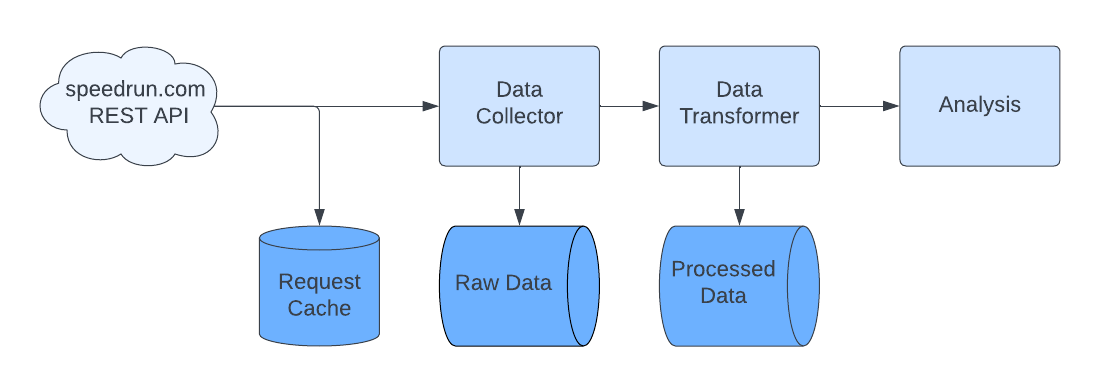
\includegraphics[width=0.8\linewidth]{images/data-pipeline.png}
    \caption{Flow of data through the collection, transformation, and analysis systems.}
    \label{fig:my_label}
\end{figure}

To satisfy the objectives of the project, data from the speedrun.com API must be collected, transformed, and analysed. There is a vast amount of data available through the speedrun.com REST API, so robust systems of collection, processing, and analysis were required to ensure the accuracy and completeness of the data, and the correctness of the analysis. 


A modular design of the three systems was chosen due to the outputs desired from each stage of the process. Specifically, the collection system requests and formats data from the speedrun.com API to be easily distributable. The transformation system processes the raw data to produce particular formats of the raw data for easy analysis. Finally, the analysis system produces data and insights from the previous stages to present and discuss in this report.

\subsection{Technology Choice}

All code from the collection to the analysis stages was written in Python. Python has a large community of users which maintain libraries that are essential for data analysis and data science. It also allows for rapid prototyping and development as it is an interpreted language with an extremely simple syntax. 


The data management and exploratory analysis used particular modules such as pandas, numpy, and matplotlib \cite{pandas, numpy, matplotlib}. These packages greatly improve the developer experience of data analysis by providing fast easy data management, mathematical operations, and chart drawing capabilities respectively. They are incredibly popular packages with a combined 291,914,314 downloads in April 2023 alone \cite{pypistats}. 


The network analysis used the networkx, graph\_tool, cdlib, and sknetwork \cite{networkx, cdlib, graph-tool, sknetwork} modules. Networkx provided many base functions such as community detection methods and basic graph analysis tools. Graph\_tool had similar functionality with increased speed, as it is implemented in C++. This package was used for particularly expensive operations, such as centrality analysis. Both cdlib and sknetwork were used for other implementations of community detection algorithms, to verify and contrast the communities generated by each implementation. 


For the game recommendation engine, sklearn was used to generate train-test splits of the transformed data due to its simple developer interface \cite{scikit-learn}.

\vspace{-5pt}
\subsection{Success Criteria}
\vspace{-5pt}

The success of the data collection system will be judged on the volume and value of the data collected from the speedrun.com API. If there is a large amount of data that is comparably accurate to the leaderboards on speedrun.com, then the collection system will be deemed successful. Likewise, the transformation and analysis systems will be successful if they provide an easy method to transform the raw data so that insights can be gathered. The transformation system must be able to create reproducible data, which is then used by the analysis system to produce valuable insights. 


The success of community detection methods will be determined both quantitatively and qualitatively. Intrinsic metrics such as modularity, performance, and coverage quantitatively determine the similarity or dissimilarity between users and games. Due to a lack of base truth for the communities of speedrun.com, extrinsic methods of evaluation cannot be used.  Modularity, performance, and coverage provide a value between 1 and 0, which are their best and worst values respectively. Additionally, the contents of the communities will determine how focused the clusters are and help determine what their commonality is.


The efficacy of the recommendation systems will also be determined both quantitatively and qualitatively. In real-world applications, metrics such as click-through rate (how many recommendations are clicked) and conversion rate (how many recommendations lead to a submitted run) determine the accuracy of these systems \cite{Cui_2021}. Creating and deploying such a system is not within the scope of this project, so we must rely on other metrics such as predicting what other games a user will play given a single game. Precision, recall, and F1-score will be used to examine how relevant the recommendations are to the users of speedrun.com. Precision measures how similar the set of recommended games and the set of played games are. Furthermore, recall measures how many games from the set of recommended games have been played by the users. The F1-score is a balanced measure between both the recall and precision. The recommendations will also be analysed to examine the diversity, accuracy, and relevance of each recommendation. Recommendation systems suffer from the ``cold-start'' problem, where lesser-known items are recommended less \cite{Eirinaki_Gao_Varlamis_Tserpes_2018}. A more diverse set of recommendations may decrease the effect of this problem. 

\subsection{Limitations of the Design}
\vspace{-5pt}

There are several limitations to the design of the project. First, a single data source is being used where there are multiple online communities of speedrunners. These other data sources may contradict each other in their community structure or user behaviour. In any case, this project provides a first impression of research in this topic. Another limitation is the lack of base truth communities of the users and games of speedrun.com. The accuracy and validity of communities must then be evaluated using internal indices, rather than comparing them to pre-labelled communities. Likewise, this project will derive hypotheses on the formation of these communities, which can be confirmed with further research. Finally, there are time and budget constraints on this project: it may not be possible to collect all necessary data as thousands of requests to the data source are needed. The design of the collection system is curated to mitigate this risk by caching requests. By publishing the data, it can be expanded upon to be included in further research.